\documentclass[12pt]{article}
\input{/Users/circle/Documents/博一下/homework/setting.tex}
\setcounter{secnumdepth}{2}

\setlength{\parindent}{2em}
\graphicspath{{../}}
\ziju{0.1pt}

%pdf文件设置
\hypersetup{
	pdfauthor={袁磊祺},
	pdftitle={统计力学及应用大作业}
}

\title{
		\vspace{-1in} 	
		\usefont{OT1}{bch}{b}{n}
		\normalfont \normalsize \textsc{\LARGE Peking University}\\[0.2cm] % Name of your university/college \\ [25pt]
		\horrule{0.5pt} \\[0.2cm]
		\huge \bfseries{统计力学及应用大作业} \\[-0.2cm]
		\horrule{2pt} \\[0.2cm]
}
\author{
		\normalfont 								\normalsize
		College of Engineering \quad 2001111690  \quad 袁磊祺\\	\normalsize
        \today
}
\date{}

\begin{document}

\input{/Users/circle/Documents/博一下/homework/setc.tex}

\maketitle

代码可在 \href{https://github.com/circlelq/Statistical-Mechanics-and-Its-Application}{https://github.com/circlelq/Statistical-Mechanics-and-Its-Application} 查看。


\section{伊辛模型简介}

伊辛模型(英语: Ising model),是一个以物理学家恩斯特·伊辛为名的数学模型,用于描述物质的铁磁性。该模型中包含了可以用来描述单个原子磁矩的参数$\sigma_i$ ,其值只能为$+1$或$-1$,分别代表自旋向上或向下,这些磁矩通常会按照某种规则排列,形成晶格,并且在模型中会引入特定交互作用的参数,使得相邻的自旋互相影响。虽然该模型相对于物理现实是一个相当简化的模型,但它却和铁磁性物质一样会产生相变。事实上,一个二维的方晶格伊辛模型是已知最简单而会产生相变的物理系统。

\section{定义}

令Λ为所有晶格点的集合,其中每个晶格点都有一个所有和它相邻的晶格点的集合(在数学上称之为图)并使这些晶格点形成一个$d$维的晶格。对于每个晶格点 $k\in$ Λ 都有一个离散变数 $\sigma_k$,其中 $\sigma_k  \in \{+1, −1\}$,代表一个晶格点的自旋。而所有变数的集合$\sigma = (\sigma_k)k\in \Lambda$则称作 自旋组态。

对于两个相邻的晶格点$i, j \in \Lambda$ ,我们可以引入一个交互作用参数Jij,此外,我们可以假设每个自旋$j\in \Lambda$都和外加的磁场 $h_j$ 作用。则整个系统的哈密顿量可写成:
\begin{equation}
	H(\sigma )=-\sum _J_{{ij}}\sigma _{i}\sigma _{j}-\mu \sum _{{j}}h_{j}\sigma_{j}
\end{equation}
其中 $<i~j>$ 代表晶格点 $i$ 和晶格点 $j$ 是相邻的的晶格点。因此哈密顿量的第一项为对每一对相邻晶格点的总和(每一对只算一次),代表所有自旋之间交互作用的能量,而第二项则是磁场和自旋交互作用的能量。$\mu$是晶格点磁矩的值,值得注意的是,电子的磁矩和他的自旋方向相反,所以哈密顿量的第二项应该要是正号比较合理,但在习惯上,还是会令第二项为负号.这里不考虑外界磁场的作用。


\section{Metropolis 方法}

用 Metropolis 方法求能量分布
\begin{equation}
	\rho = \me^{-E/T},
	\label{eq:1}
\end{equation}
其中
\begin{equation}
	E = \sum_i J \sigma_i \sigma_{i+1}, \quad J = \pm 1.
\end{equation}
粒子指向向上时$\sigma_i=1$,向下时, $\sigma_i=-1$。

\begin{enumerate}
	\item 相点初始位置为50个点,全部向上,取周期边界条件计算其能量.
	\item 若指向状态为$x_1$,有两种方式改变状态:
	      \begin{itemize}
		      \item 随机选择一个点,改变其指向,
		      \item 或者随机选取一段区域,改变其指向。
	      \end{itemize}
	\item 根据\cref{eq:1}来计算其概率密度。
	      \begin{enumerate}
		      \item 若$\rho_2>\rho_1$,则相点移动到$x_2$。
		      \item 若$\rho_2<\rho_1$,则产生一个$[0,1]$中的随机数$\xi$,若$\xi<\me^{-(E_2-E_1)/T}$则相点移动到$x_2$。否则不移动。
	      \end{enumerate}
	\item 重复2,3,直到给定的停止条件。
\end{enumerate}

\section{模拟结果}

分别考虑$J=1,-1$两种情况。

当$J=1$时为竞争关系, 如\cref{fig:Es,fig:Eb} 所示,分别为每次变动一个点和每次变动一个区域内的点的结果。取$N=1\times 10^7$次模拟。可以发现两种方法获得的$\sigma_i$变化基本相同。

当温度$T$较小时,$\sigma_i$基本保持为0,当温度$T$增大时,$\sigma_i$的震荡开始增加。


\begin{figure}
	\centering
	\begin{subfigure}[b]{0.49\textwidth}
		\centering
		\includegraphics[width=\textwidth]{fig1DJ1N1e7/sig_s_T0.1J1.pdf}
		\caption{$T=0.1$}
	\end{subfigure}
	\hfill
	\begin{subfigure}[b]{0.49\textwidth}
		\centering
		\includegraphics[width=\textwidth]{fig1DJ1N1e7/sig_s_T0.2J1.pdf}
		\caption{$T=0.2$}
	\end{subfigure}
	\hfill
	\begin{subfigure}[b]{0.49\textwidth}
		\centering
		\includegraphics[width=\textwidth]{fig1DJ1N1e7/sig_s_T0.5J1.pdf}
		\caption{$T=0.5$}
	\end{subfigure}
	\begin{subfigure}[b]{0.49\textwidth}
		\centering
		\includegraphics[width=\textwidth]{fig1DJ1N1e7/sig_s_T1J1.pdf}
		\caption{$T=1$}
	\end{subfigure}
	\begin{subfigure}[b]{0.49\textwidth}
		\centering
		\includegraphics[width=\textwidth]{fig1DJ1N1e7/sig_s_T2J1.pdf}
		\caption{$T=2$}
	\end{subfigure}
	\caption{每次变动一个点。$J=1$.}
	\label{fig:Es}
\end{figure}



\begin{figure}
	\centering
	\begin{subfigure}[b]{0.49\textwidth}
		\centering
		\includegraphics[width=\textwidth]{fig1DJ1N1e7/sig_b_T0.1J1.pdf}
		\caption{$T=0.1$}
	\end{subfigure}
	\hfill
	\begin{subfigure}[b]{0.49\textwidth}
		\centering
		\includegraphics[width=\textwidth]{fig1DJ1N1e7/sig_b_T0.2J1.pdf}
		\caption{$T=0.2$}
	\end{subfigure}
	\hfill
	\begin{subfigure}[b]{0.49\textwidth}
		\centering
		\includegraphics[width=\textwidth]{fig1DJ1N1e7/sig_b_T0.5J1.pdf}
		\caption{$T=0.5$}
	\end{subfigure}
	\begin{subfigure}[b]{0.49\textwidth}
		\centering
		\includegraphics[width=\textwidth]{fig1DJ1N1e7/sig_b_T1J1.pdf}
		\caption{$T=1$}
	\end{subfigure}
	\begin{subfigure}[b]{0.49\textwidth}
		\centering
		\includegraphics[width=\textwidth]{fig1DJ1N1e7/sig_b_T2J1.pdf}
		\caption{$T=2$}
	\end{subfigure}
	\caption{每次变动一个区域内的点。$J=1$.}
	\label{fig:Eb}
\end{figure}


当$J=-1$时为合作关系,如\cref{fig:EsJ-1,fig:EbJ-1} 所示,当每次变动一个点时,$T=0.1,0.2$时$\sigma_i$都保持为1不变,而当$T\leq 0.5$时,$\sigma_i$开始在$[-1,1]$之间震荡。而当$T=2$时,震荡的范围缩小了。

对于区域反转,$T$较小时,在$[-1,1]$之间震荡,并且都达到了$1,-1$,而当$T=1,2$时,震荡的范围缩小了。



\begin{figure}
	\centering
	\begin{subfigure}[b]{0.49\textwidth}
		\centering
		\includegraphics[width=\textwidth]{fig1DJ1N1e7/sig_s_T0.1J-1.pdf}
		\caption{$T=0.1$}
	\end{subfigure}
	\hfill
	\begin{subfigure}[b]{0.49\textwidth}
		\centering
		\includegraphics[width=\textwidth]{fig1DJ1N1e7/sig_s_T0.2J-1.pdf}
		\caption{$T=0.2$}
	\end{subfigure}
	\hfill
	\begin{subfigure}[b]{0.49\textwidth}
		\centering
		\includegraphics[width=\textwidth]{fig1DJ1N1e7/sig_s_T0.5J-1.pdf}
		\caption{$T=0.5$}
	\end{subfigure}
	\begin{subfigure}[b]{0.49\textwidth}
		\centering
		\includegraphics[width=\textwidth]{fig1DJ1N1e7/sig_s_T1J-1.pdf}
		\caption{$T=1$}
	\end{subfigure}
	\begin{subfigure}[b]{0.49\textwidth}
		\centering
		\includegraphics[width=\textwidth]{fig1DJ1N1e7/sig_s_T2J-1.pdf}
		\caption{$T=2$}
	\end{subfigure}
	\caption{每次变动一个点。$J=-1$.}
	\label{fig:EsJ-1}
\end{figure}



\begin{figure}
	\centering
	\begin{subfigure}[b]{0.49\textwidth}
		\centering
		\includegraphics[width=\textwidth]{fig1DJ1N1e7/sig_b_T0.1J-1.pdf}
		\caption{$T=0.1$}
	\end{subfigure}
	\hfill
	\begin{subfigure}[b]{0.49\textwidth}
		\centering
		\includegraphics[width=\textwidth]{fig1DJ1N1e7/sig_b_T0.2J-1.pdf}
		\caption{$T=0.2$}
	\end{subfigure}
	\hfill
	\begin{subfigure}[b]{0.49\textwidth}
		\centering
		\includegraphics[width=\textwidth]{fig1DJ1N1e7/sig_b_T0.5J-1.pdf}
		\caption{$T=0.5$}
	\end{subfigure}
	\begin{subfigure}[b]{0.49\textwidth}
		\centering
		\includegraphics[width=\textwidth]{fig1DJ1N1e7/sig_b_T1J-1.pdf}
		\caption{$T=1$}
	\end{subfigure}
	\begin{subfigure}[b]{0.49\textwidth}
		\centering
		\includegraphics[width=\textwidth]{fig1DJ1N1e7/sig_b_T2J-1.pdf}
		\caption{$T=2$}
	\end{subfigure}
	\caption{每次变动一个区域内的点。$J=-1$.}
	\label{fig:EbJ-1}
\end{figure}


\begin{figure}
	\centering
	\begin{subfigure}[b]{0.49\textwidth}
		\centering
		\includegraphics[width=\textwidth]{fig1DJ1N1e7/ave_sJ-1.pdf}
		\caption{Single, $J=-1$}
	\end{subfigure}
	\hfill
	\begin{subfigure}[b]{0.49\textwidth}
		\centering
		\includegraphics[width=\textwidth]{fig1DJ1N1e7/ave_sJ1.pdf}
		\caption{Single, $J=1$}
	\end{subfigure}
	\hfill
	\begin{subfigure}[b]{0.49\textwidth}
		\centering
		\includegraphics[width=\textwidth]{fig1DJ1N1e7/ave_bJ-1.pdf}
		\caption{Block, $J=-1$}
	\end{subfigure}
	\begin{subfigure}[b]{0.49\textwidth}
		\centering
		\includegraphics[width=\textwidth]{fig1DJ1N1e7/ave_bJ1.pdf}
		\caption{Block, $J=1$}
	\end{subfigure}
	\caption{$J=-1,\ 1$时$<\sigma_i>$随$T$的变化关系.}
	\label{fig:1Dave}
\end{figure}



\section{2D Ising 模型}

对于二维 Ising 模型,
\begin{equation}
	E = -J \sum_i \sigma_i \sigma_{i'}.
\end{equation}
其中$i'$表示临近的点。

\subsection{Wolff 算法}

Wolff 算法的过程如下

\begin{enumerate}
	\item 随机选择一个格点。
	\item 依次看所取格点的周边,如果是同向的相邻点,则以
	      \begin{equation}
		      P_{\mathrm{add}} = 1 - \me^{-2\beta J},
	      \end{equation}
	      的概率加入集团。其中$\beta=\frac{1}{T},\ J=1$.
	\item 对新加入的格点重复步骤2,知道形成一个最大的集团。
	\item 直接反转集团中所有格点的方向。
\end{enumerate}

通过理论分析可知这样的过程将满足
\begin{equation}
	\frac{T(\mu\to\nu)A(\mu\to\nu)}{T(\nu\to\mu)A(\nu\to\mu)} = \me^{-\beta\left(E_{\nu}-E_{\mu}\right)}.
\end{equation}
其中$\mu,\nu$分别为初态和末态。网格是$20\times 20$,周期边界条件。当$T(0\to 5J)$时,画出$<\sigma>$和$T$的关系。

如\cref{fig:2Dmeansig} 所示为二维格点$<\sigma_i>$随迭代次数的变化关系, $J=1$,迭代$1\times 10^{6}$次.当$T$较小时, $<\sigma_i>$在$[-1,1]$之间震荡, $T$增大后,震荡范围减小。如\cref{fig:2DsigT} 所示,为当$T(0\to 5J)$时, $<\sigma>$和$T$的关系。其中$<\sigma>$取了绝对值,可以发现$<\sigma>$随$T$的增加而增大。

\begin{figure}
	\centering
	\begin{subfigure}[b]{0.49\textwidth}
		\centering
		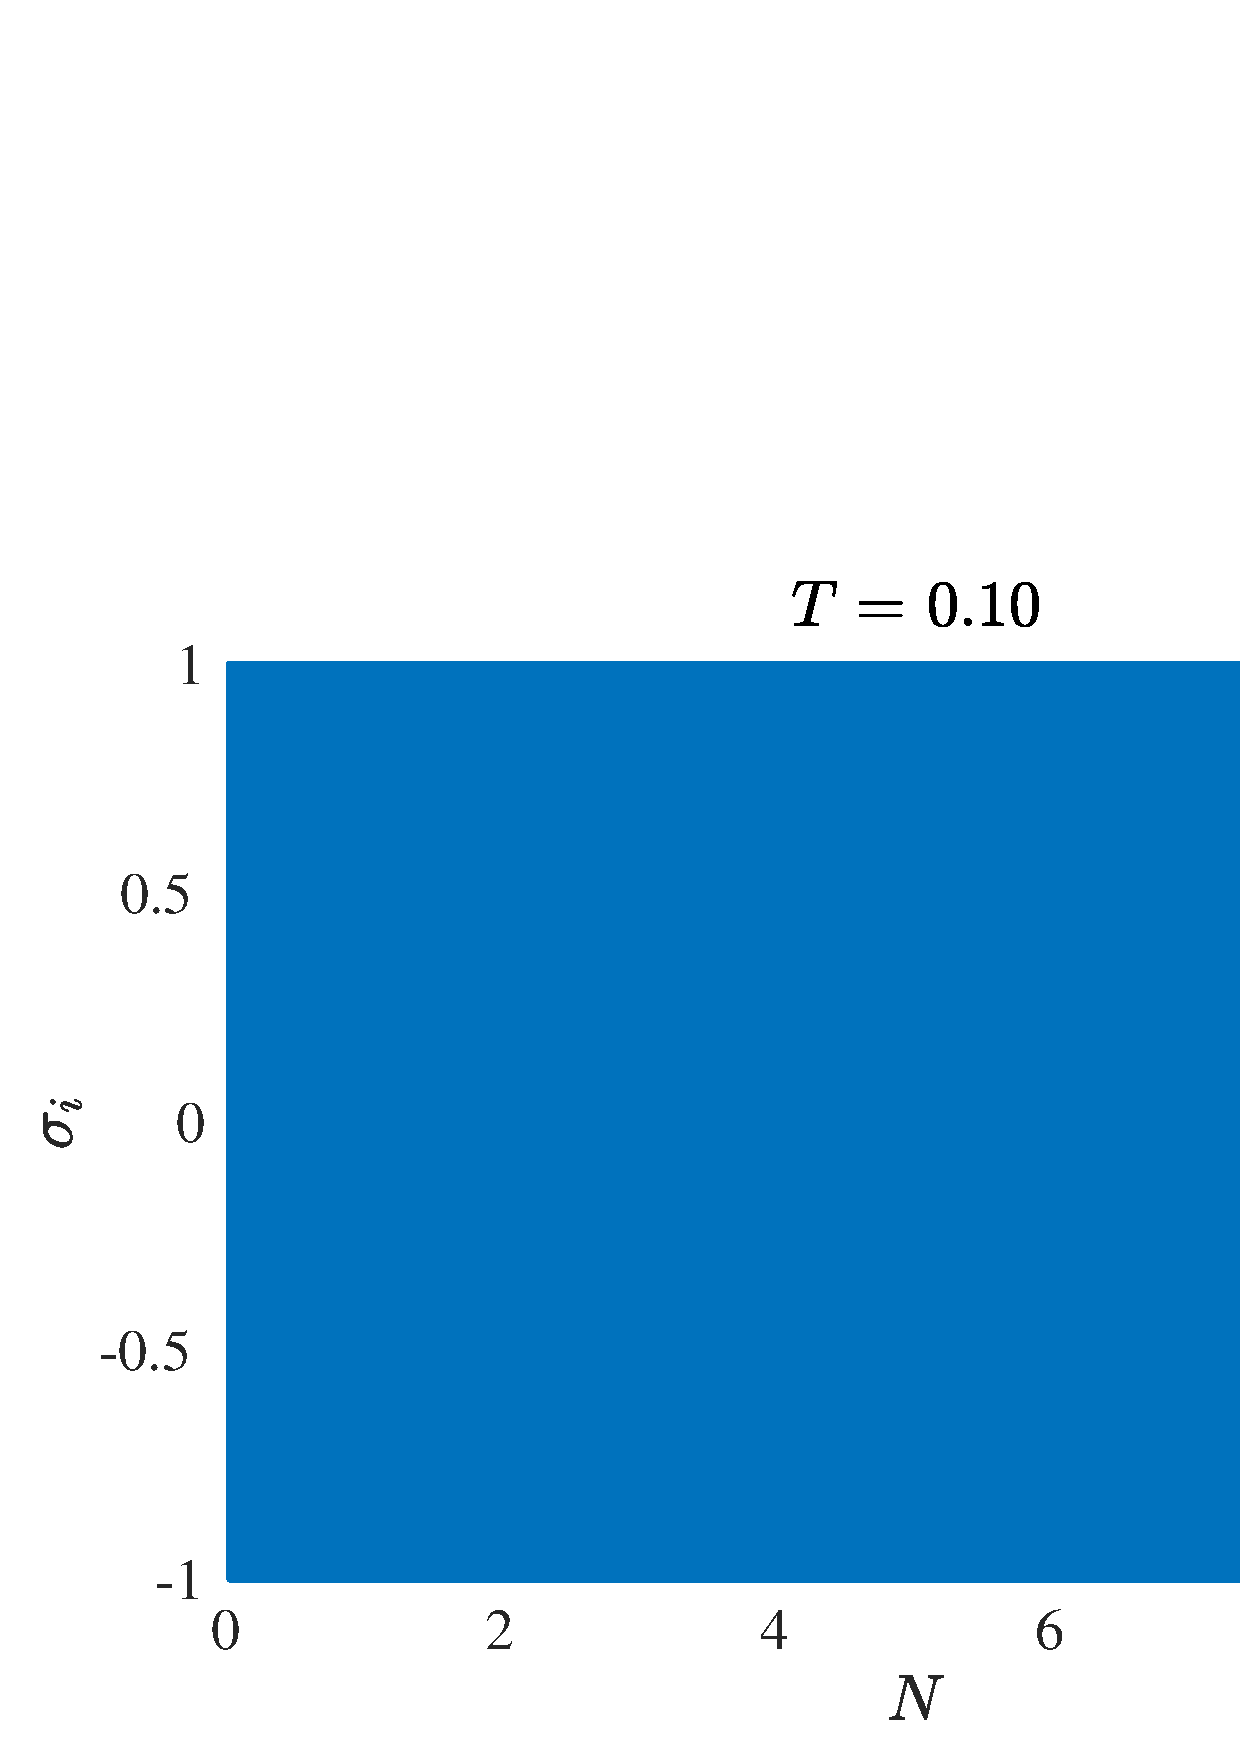
\includegraphics[width=\textwidth]{2D/2D1e7/meansigT0.1.pdf}
		\caption{$T=0.1$}
	\end{subfigure}
	\hfill
	\begin{subfigure}[b]{0.49\textwidth}
		\centering
		\includegraphics[width=\textwidth]{2D/2D1e7/meansigT1.pdf}
		\caption{$T=0.2$}
	\end{subfigure}
	\hfill
	\begin{subfigure}[b]{0.49\textwidth}
		\centering
		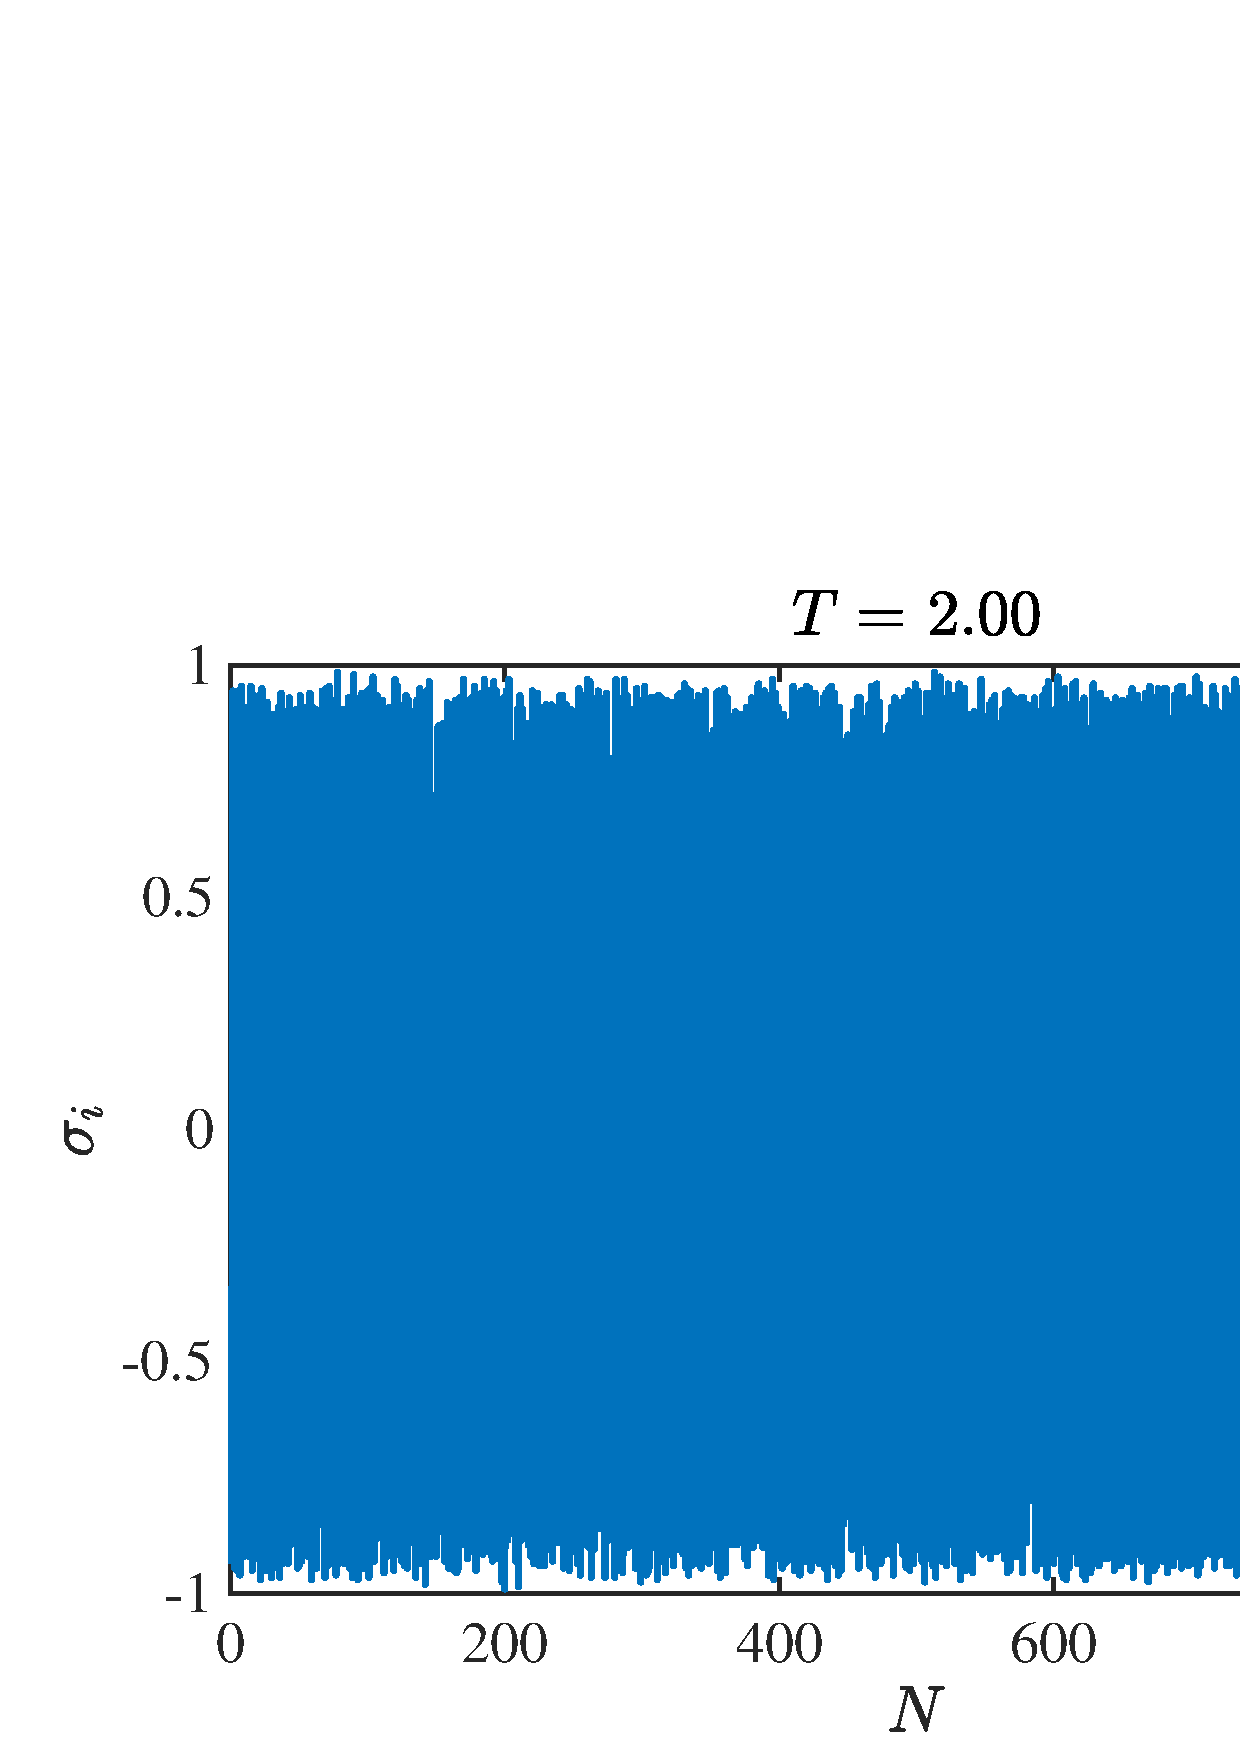
\includegraphics[width=\textwidth]{2D/2D1e7/meansigT2.pdf}
		\caption{$T=0.5$}
	\end{subfigure}
	\begin{subfigure}[b]{0.49\textwidth}
		\centering
		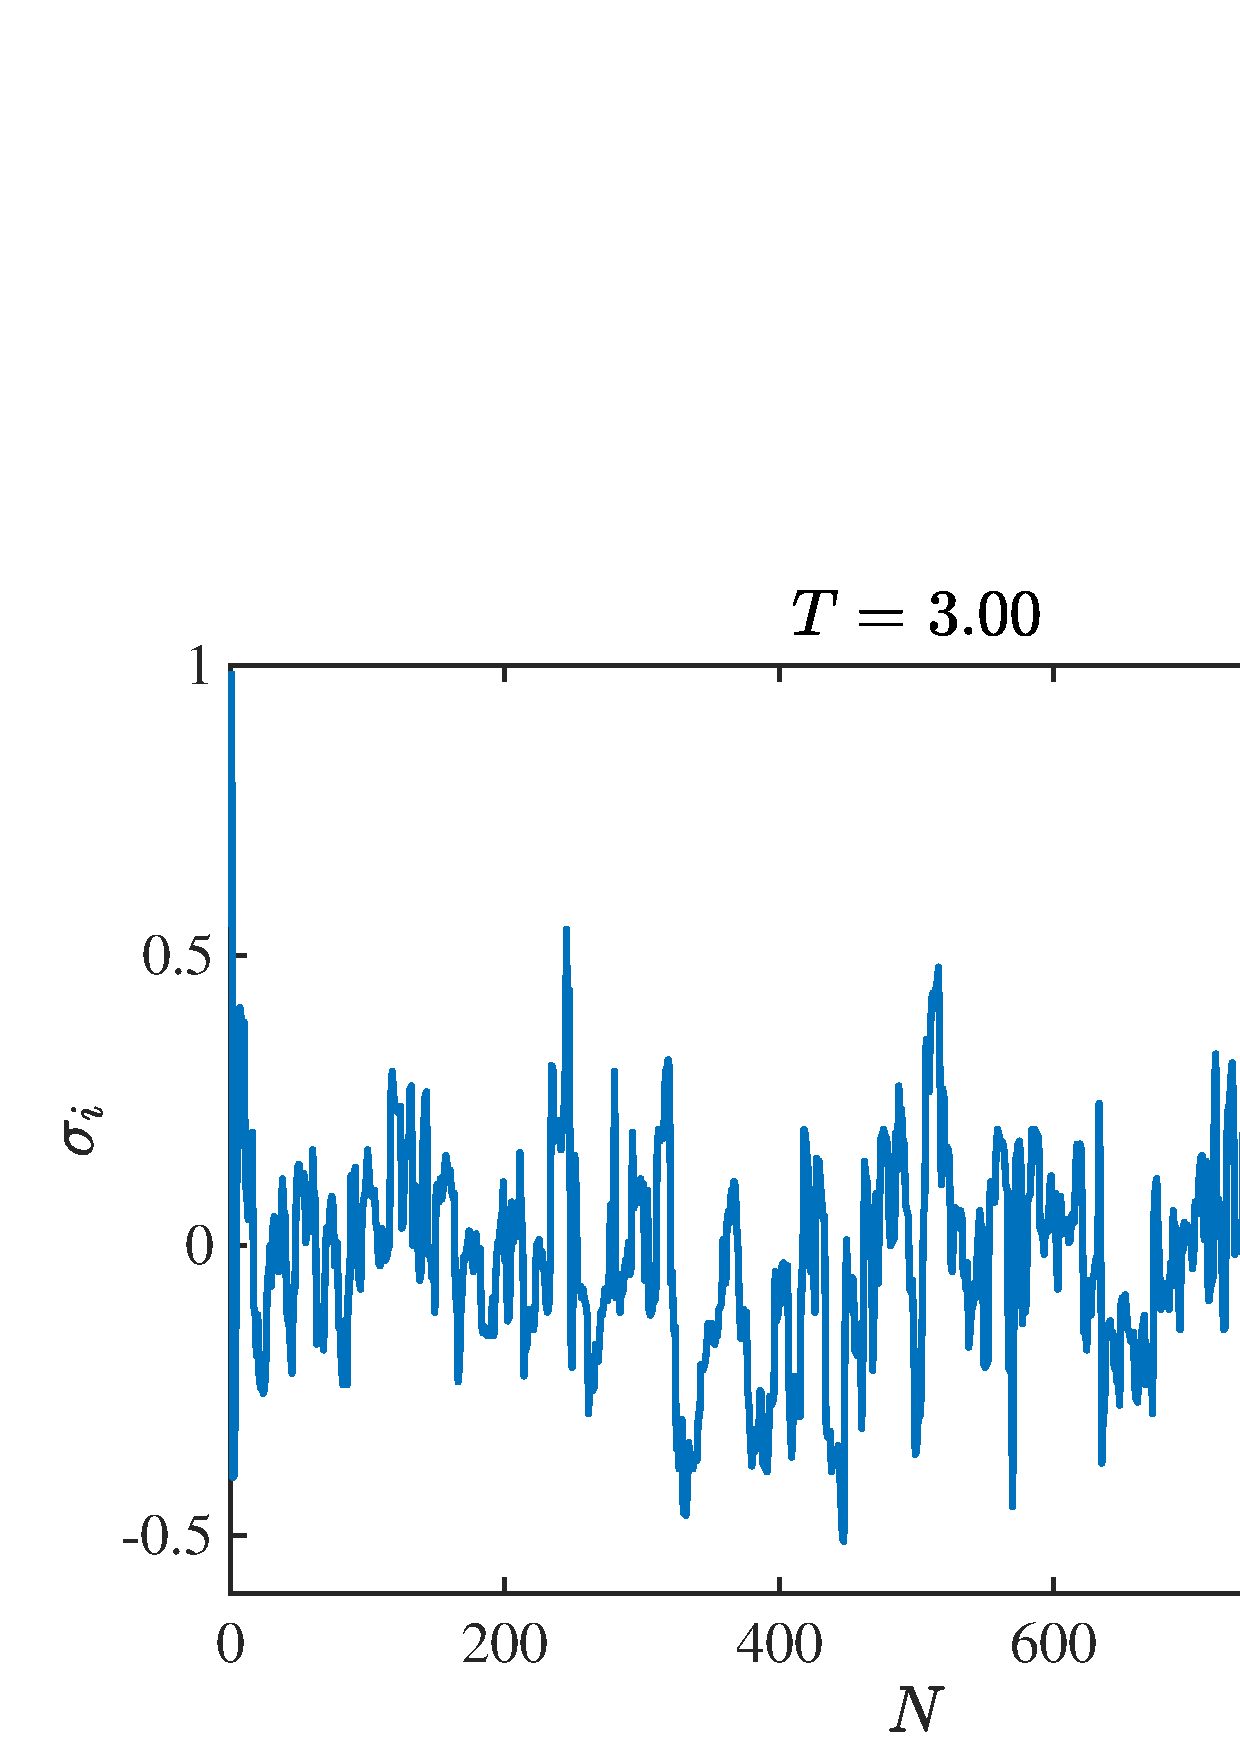
\includegraphics[width=\textwidth]{2D/2D1e7/meansigT3.pdf}
		\caption{$T=1$}
	\end{subfigure}
	\hfill
	\begin{subfigure}[b]{0.49\textwidth}
		\centering
		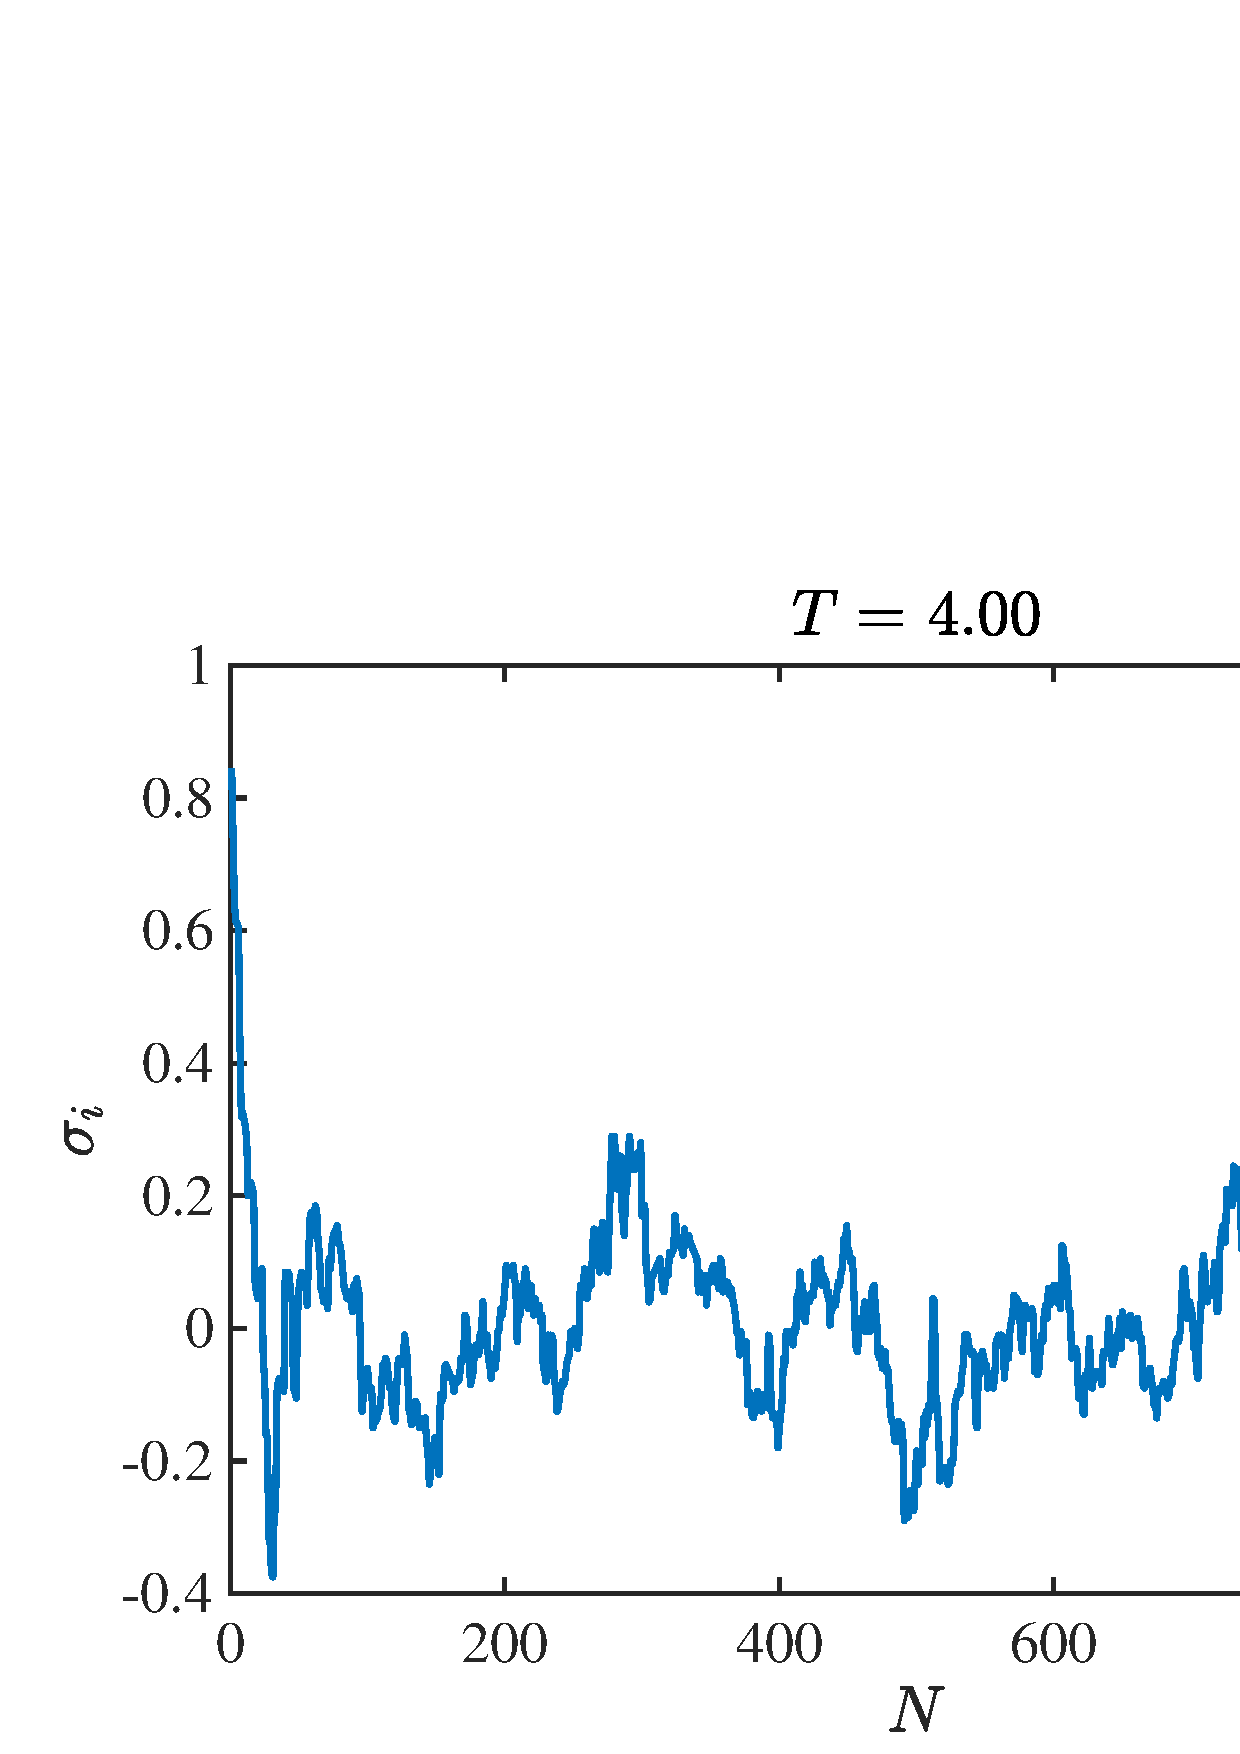
\includegraphics[width=\textwidth]{2D/2D1e7/meansigT4.pdf}
		\caption{$T=2$}
	\end{subfigure}
	\begin{subfigure}[b]{0.49\textwidth}
		\centering
		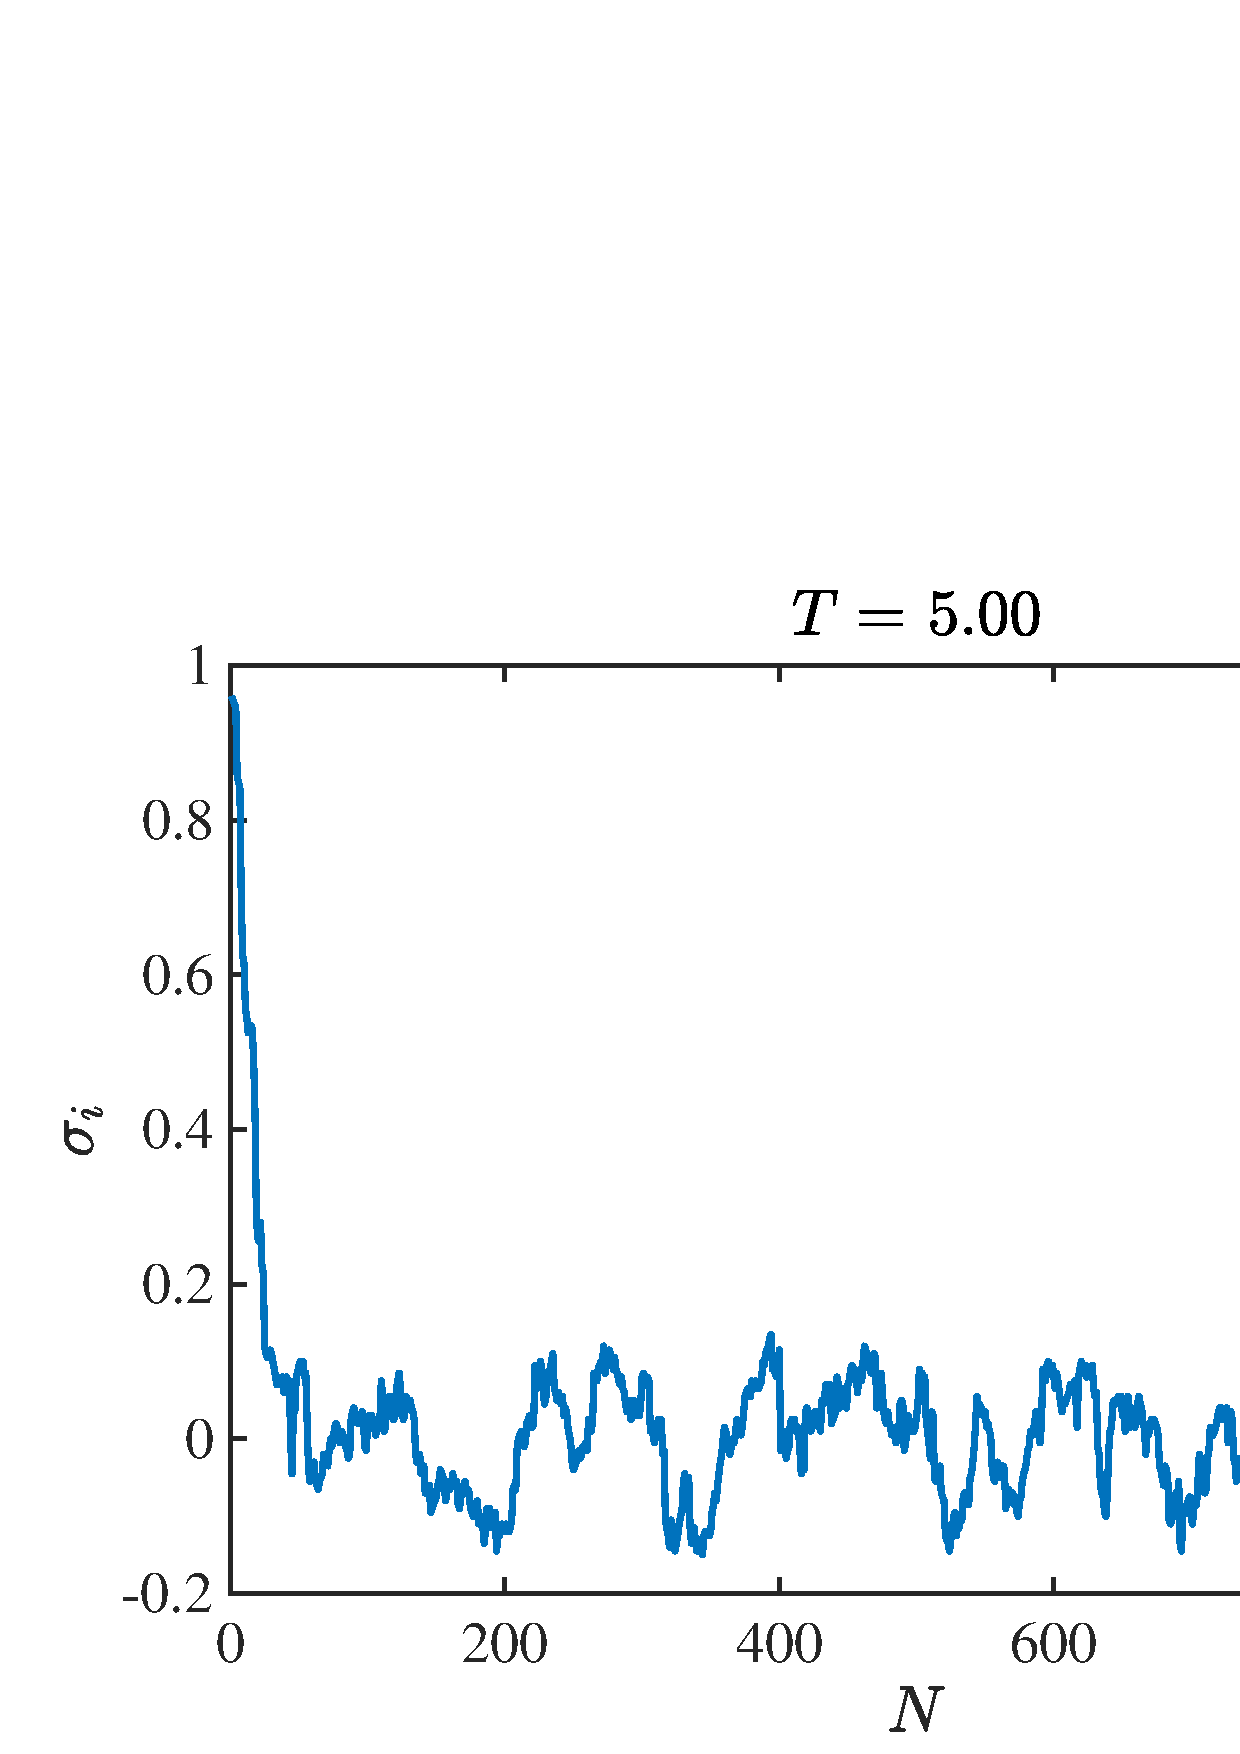
\includegraphics[width=\textwidth]{2D/2D1e7/meansigT5.pdf}
		\caption{$T=2$}
	\end{subfigure}
	\caption{二维格点$<\sigma_i>$随迭代次数的变化关系, $J=1$.}
	\label{fig:2Dmeansig}
\end{figure}

\begin{figure}[htp]
	\centering
	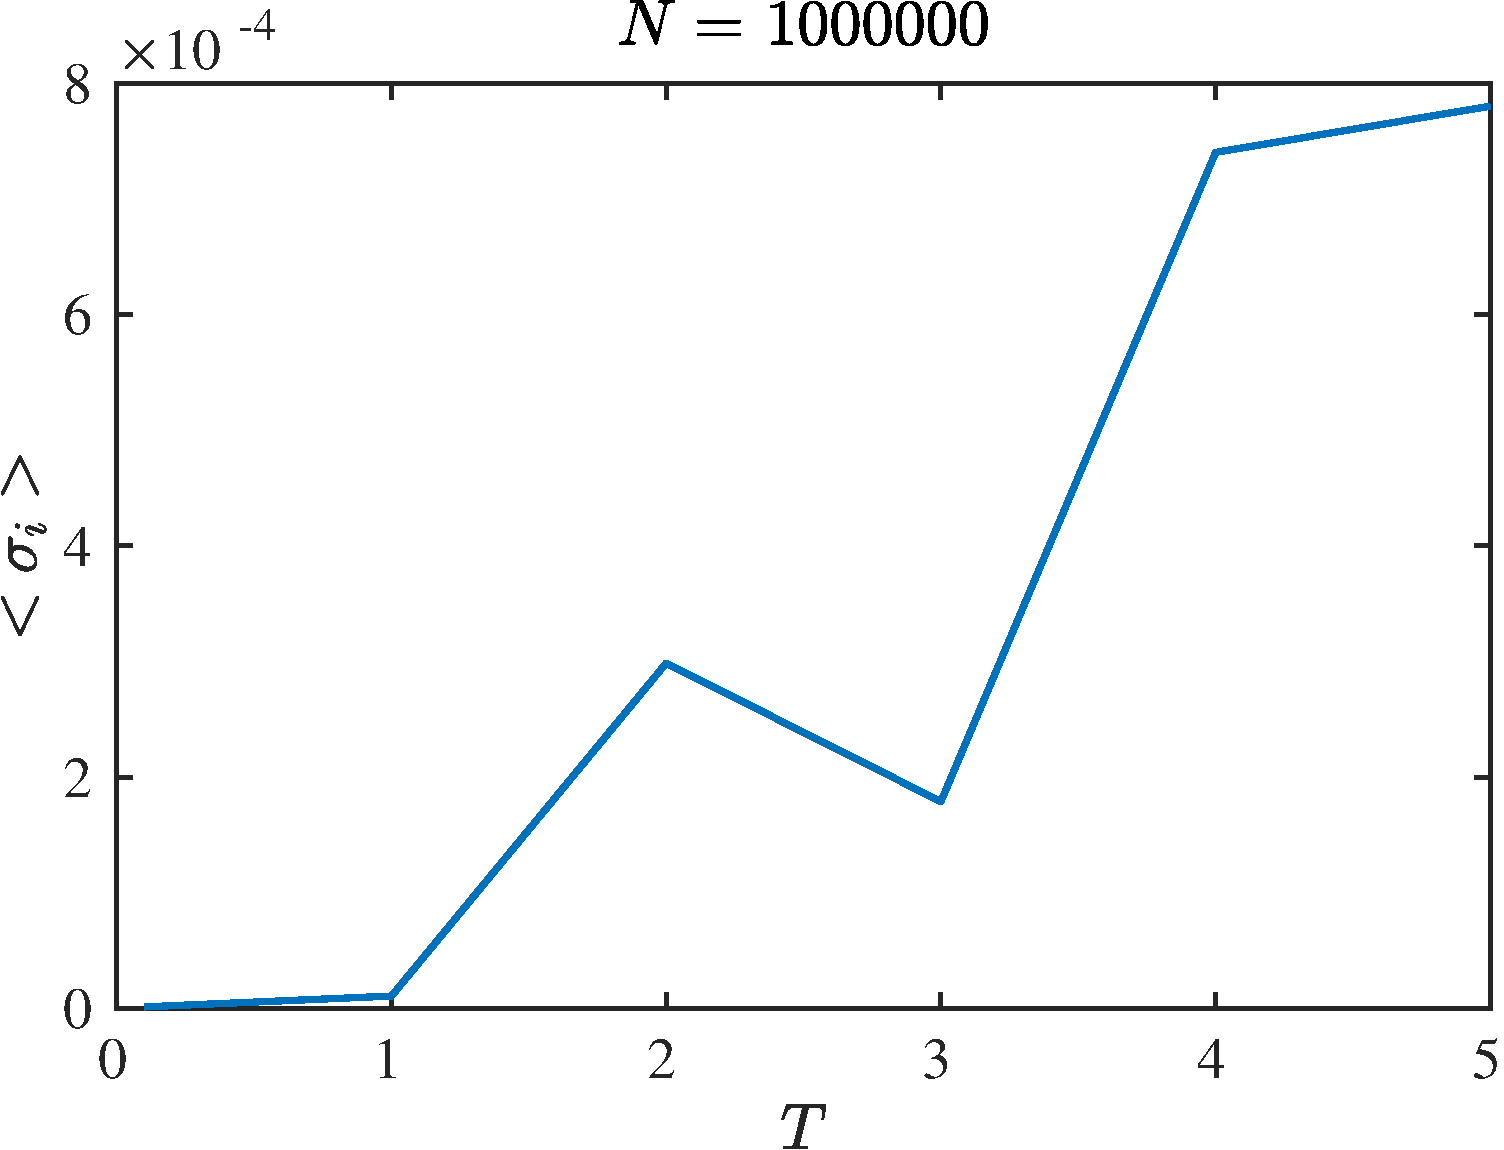
\includegraphics[width=12cm]{2D/2D1e7/avesig.pdf}
	\caption{$<\sigma_i>$随$T$的变化关系。}
	\label{fig:2DsigT}
\end{figure}





% \nocite{*}

% \input{bib.tex}

\end{document}

